\documentclass[11pt]{article}

% Load packages
\usepackage{float} % for formatting figures
\usepackage{amsmath, amsfonts} % for math
\usepackage{graphicx} % for figures
\usepackage[margin=1in]{geometry} % to set margins
\usepackage{tcolorbox} % to create nice boxes
\tcbuselibrary{skins,breakable} % extra libraries for the nice boxes
\usepackage{listings}
\usepackage{enumerate}
\usepackage{empheq}

% Define a custom box for the solutions. Don't change this!
\newtcolorbox[]{solution}
    {colframe=red!20, 
        colback=white, 
        sharp corners,
        title=Solution,
        enhanced,
        coltitle=black,
        fonttitle=\bfseries,
        attach boxed title to top left={yshift*=-\tcboxedtitleheight/2, xshift=3mm},
        boxed title style={sharp corners, colback=red!20}
        }

% This package is not installed
%\usepackage{boondox-calo}

\newcommand{\lr}[1]{\left(#1\right)}

\usepackage{hyperref}
\hypersetup{
    colorlinks=true,
    linkcolor=blue,
    filecolor=magenta,      
    urlcolor=cyan
}

\title{Homework 2 \\[1.0em] \normalsize Due Monday, April 15th at 11:59 PM}
\date{}


% Write the document
\begin{document}

  \maketitle

  \section{Problem 1:  Channel Flow with a central narrowing}

Simulating channel flow in 2D with a narrowing is the target.

The type of flow in absence of the narrowing is the well-known Hagen-Poiseuille flow 
(and by the way, Poiseuille was a physicist and physiologist who studied blood flows 
in a systematic way). Let's write the corresponding grid for a straight channel aligned along, say, the x axis. 

When constructing the grid and using it in the LBM context 
you should apply what you have learned about grid management. Let's recall that in absence of open boundaries (inlet or outlet), each fluid node should always 
be surrounded by other fluid or wall nodes to preserve mass and momentum locally (no leakage rule).

The solution should employ two different options:

    \begin{enumerate}
      \item A periodic channel (aligned with the x direction): start from a quiescent fluid and
      apply a body acceleration uniformly through the fluid until you match the Reynolds number at steady state.
      \item A non-periodic channel with inlet and outlet faces and by applying a uniform velocity 
      at inlet and outlet with plug flow profiles.
    \end{enumerate}

    Use no-slip boundary conditions at the walls and a Reynolds number of $10^{-2}$ computed from fluid velocity 
    imposed at $x=0$ (the inlet region for non-period channel) and characterstic length being $H$.

    \begin{figure}[h!]
      \centering{}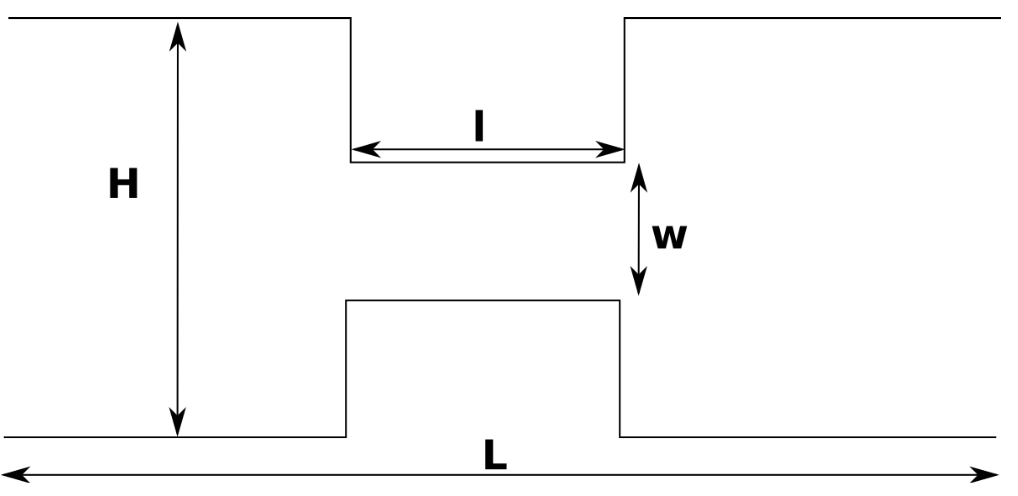
\includegraphics[scale=0.6]{narrowing}
      \caption{The geometry for the channel with central narrowing.}
      \label{fig:narrowing}
    \end{figure}

\begin{solution} 

We first need to ensure a Reynolds number of $10^{-2}$.

The Reynolds number is computed by

    \begin{align*}
      Re = \frac{uH}{\nu}
    \end{align*}

The characteristic length $H = 60$ here. $u$ is set to be the velocity at $x=0$. $\nu$ is the kinematic viscosity, computed from 
    \begin{align*}
        \nu = c_s^2 (\frac{1}{\Omega} - \frac{1}{2})
    \end{align*}

where $c_s^2 = \frac{1}{3}$ is sound speed squared. $\Omega$ is the relaxation frequency in BGK operator. In our code, we set $\Omega = 1$, indicating a full-relaxation scheme (except for the last question that requires changing $\Omega$). Thus $\nu = \frac{1}{2} c_s^2 = 1/6$.

The desired $u$ can be computed from
    \begin{align*}
          u & = \frac{Re \cdot \nu}{H} \\
            & = \frac{0.01 \cdot 1/6}{60} \\
            & = 2.8 \times 10^{-5}
    \end{align*}

For periodic boundary (case 1), we tweak forcing so that the steady $u(x=0)$ is around  $2.8 \times 10^{-5}$. We find the forcing to be $1 \times 10^{-8}$. For non-periodic boundary, we directly apply this velocity to the boundary grid points. Both cases achieve steady state in about 8000 time steps.

\end{solution}
    
    \textbf{For a fixed set of values for the geometry 
    as in Fig. \ref{fig:narrowing}, (suggested values $L=200$, $H=60$, $l=50$, $w=30$), 
    calculate the following quantities:}
    \begin{enumerate}
      \item The pressure field
      \item The velocity field 
      \item The volume flow rate 
      \item The average and maximum velocities in the channel
    \end{enumerate}

\graphicspath{ {./JiaweiZhuang/HW2_figures/basic_variables/} }

\begin{solution} 

The pressure is computed from

    \begin{align*}
        p &= c_s^2 \rho= \frac{1}{3} \rho
    \end{align*}

Fig \ref{fig:macro_case1} and Fig \ref{fig:macro_case2} show the macroscopic fields with the periodic (case 1) and non-periodic (case 2) boundary conditions.

\textbf{Periodic Boundary Conditions}

\begin{figure}[H]
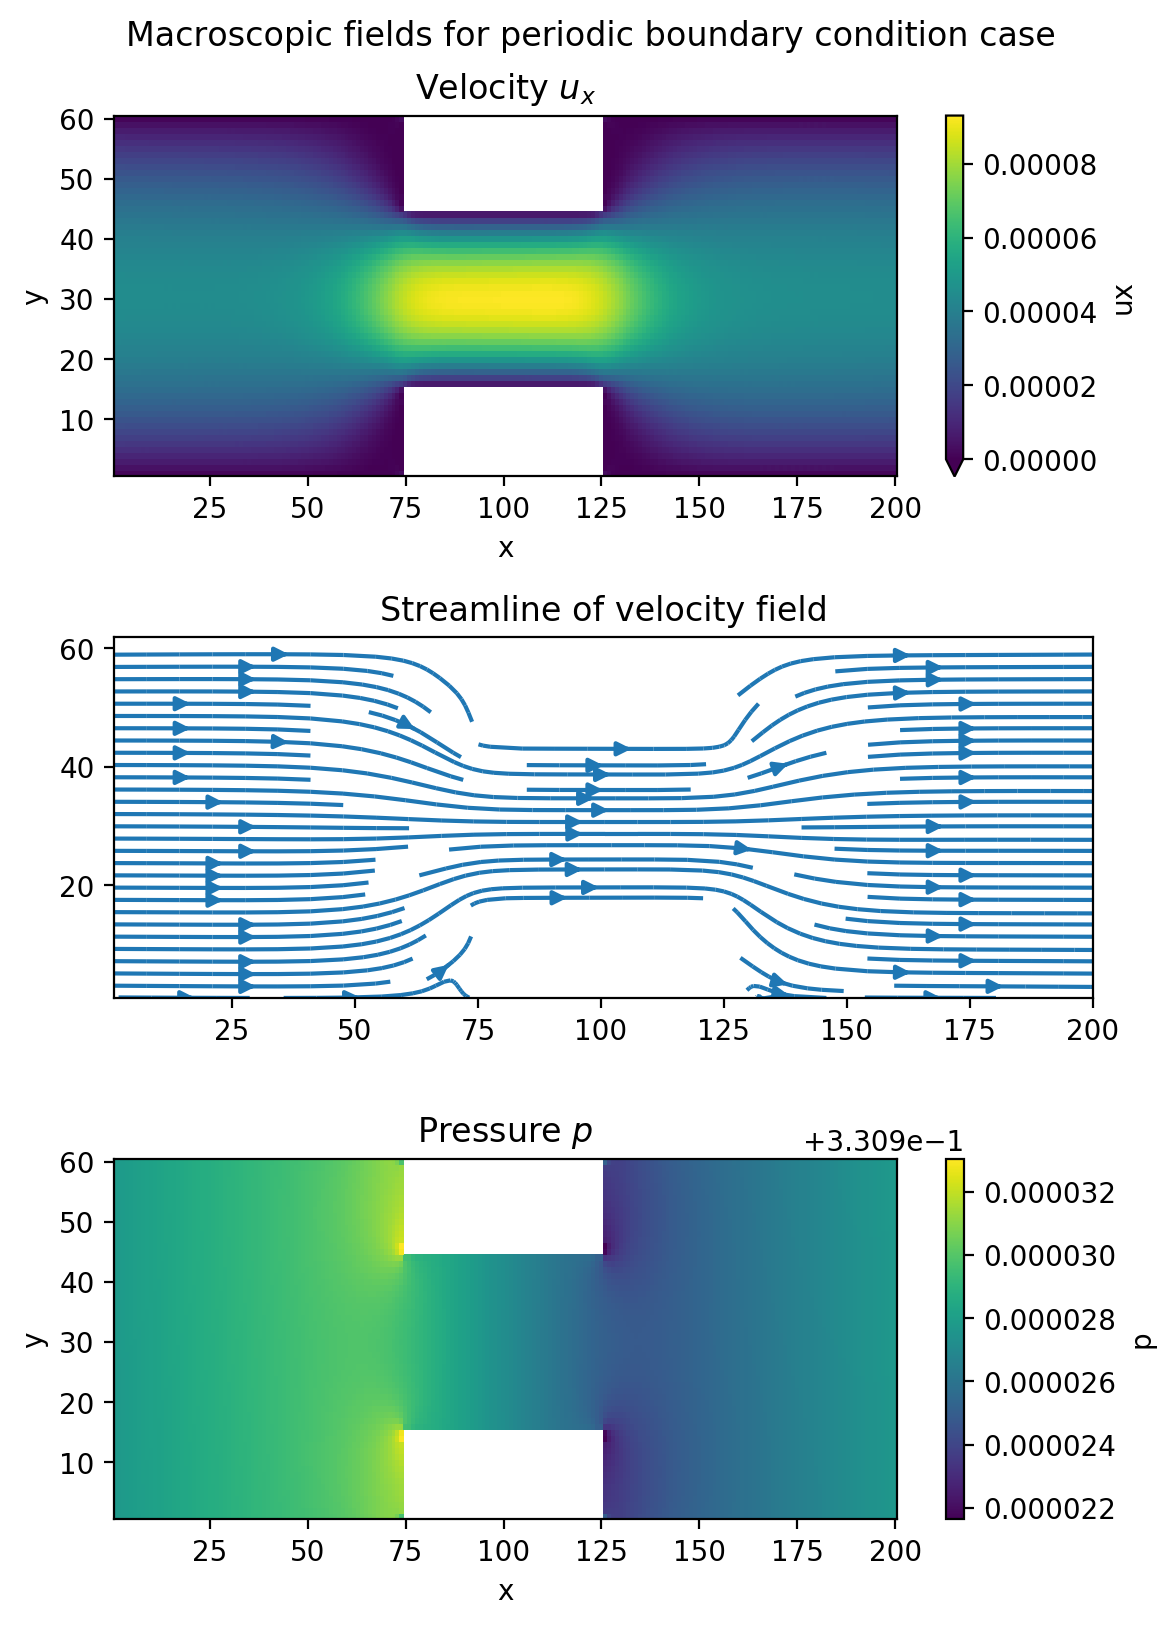
\includegraphics[scale=0.76]{case1_2d_fields}
\centering
\caption{Macroscopic variables for periodic boundary case}
\label{fig:macro_case1}
\end{figure}

\end{solution}

\begin{solution} 
\textbf{Imposed Boundary Conditions}

\begin{figure}[H]
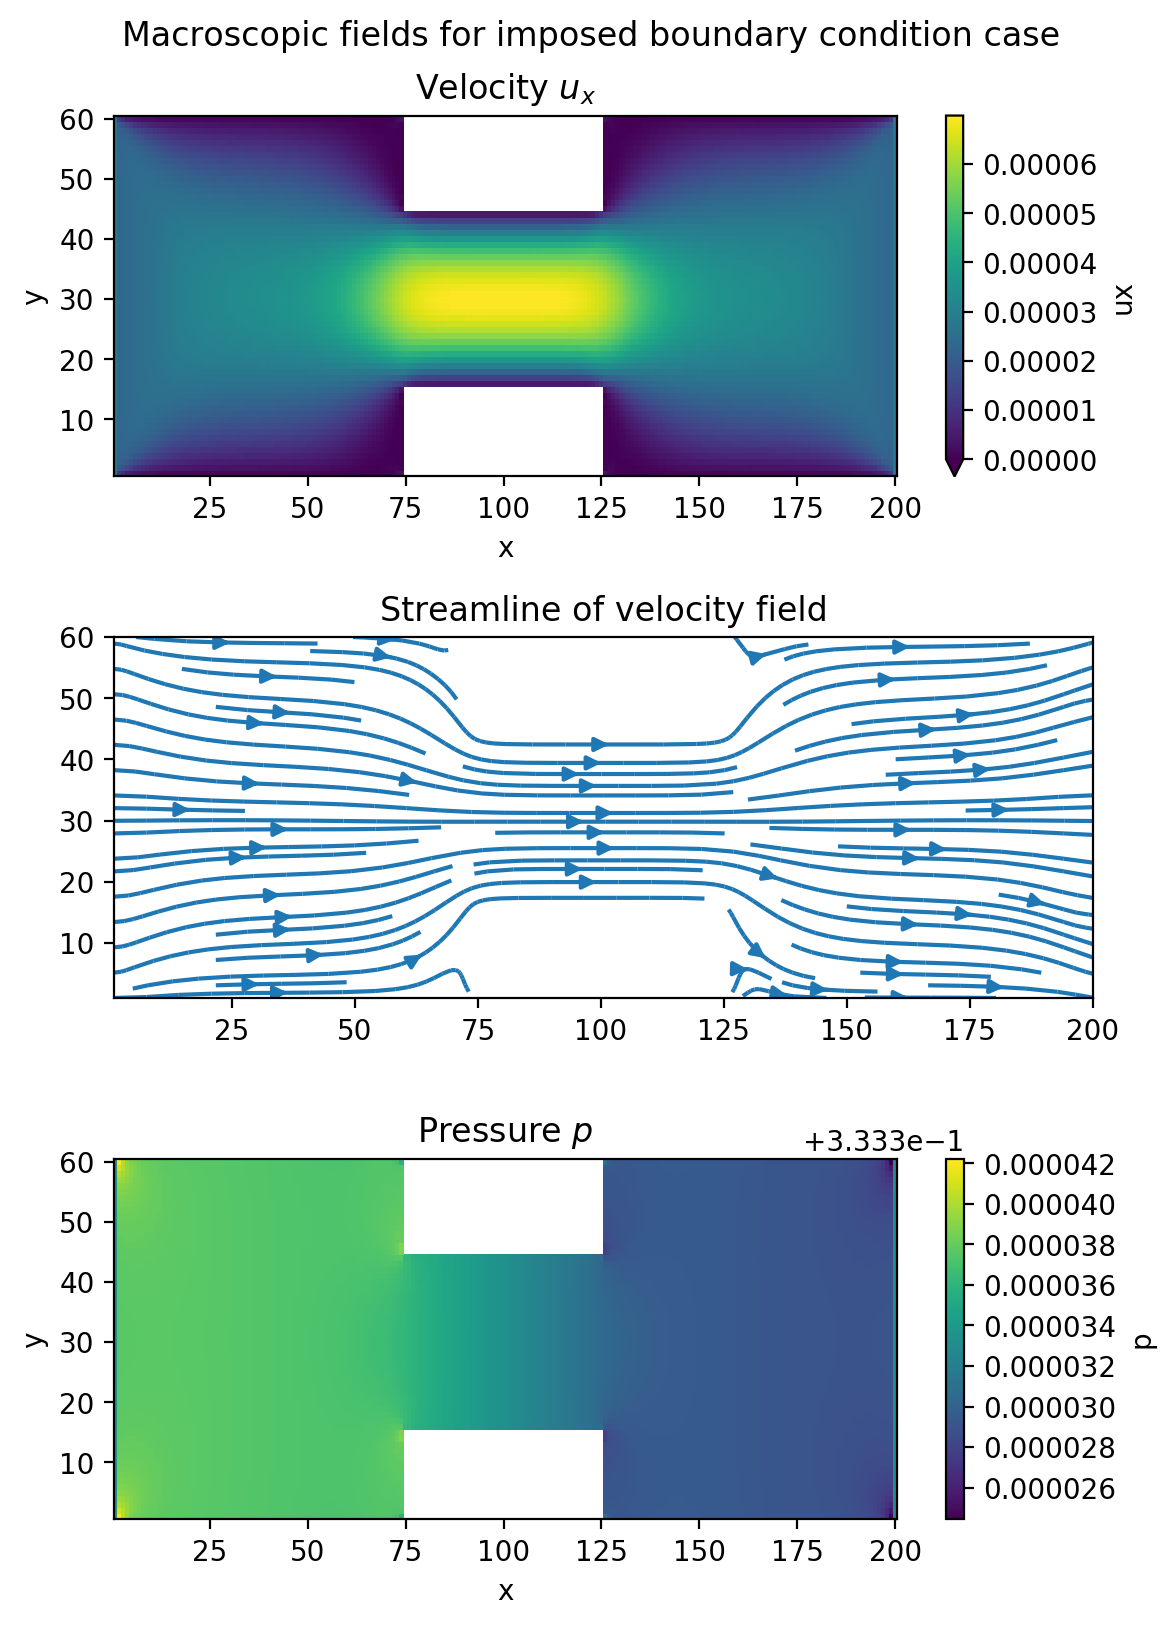
\includegraphics[scale=0.76]{case2_2d_fields}
\centering
\caption{Macroscopic variables for non-periodic boundary case}
\label{fig:macro_case2}
\end{figure}

\end{solution}

\begin{solution} 
\textbf{Volume Flow Rate}

The volume flow rates can be computed from the integral over x, on a specific cross-section $x=x_i$. Fig \ref{fig:flow_case1} and Fig \ref{fig:flow_case2} show the volume flow rate at all possible $x$, for two different boundary conditions. The rate is roughly constant at different $x$. For boundary case 1, $rate \approx 0.0018$; for boundary case 1, $rate \approx 0.0014$.

\begin{figure}[H]
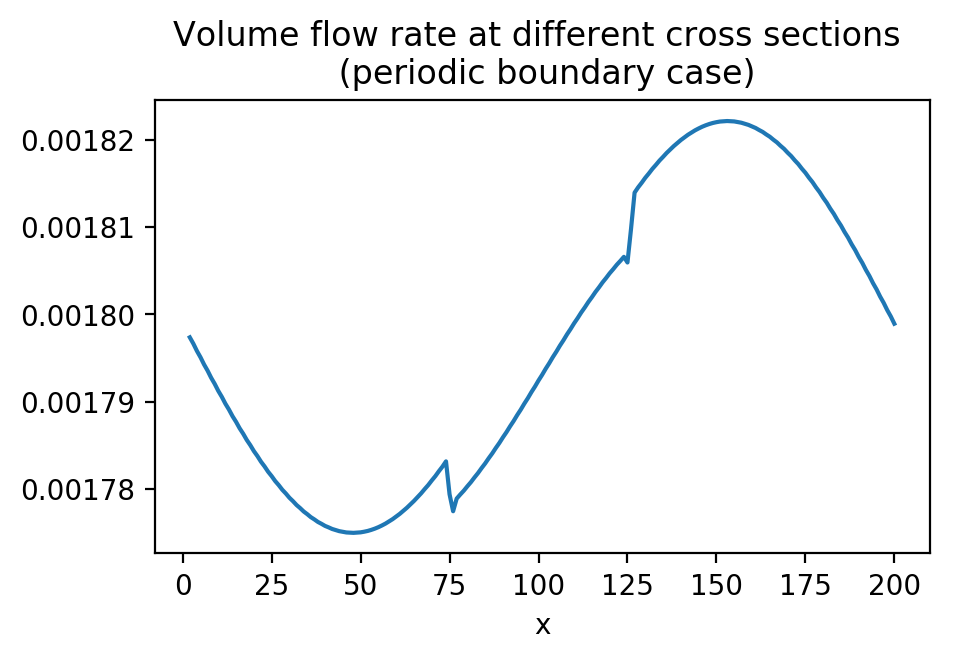
\includegraphics[scale=0.8]{case1_volume_flow}
\centering
\caption{Volume flow rates for periodic boundary case}
\label{fig:flow_case1}
\end{figure}

\begin{figure}[H]
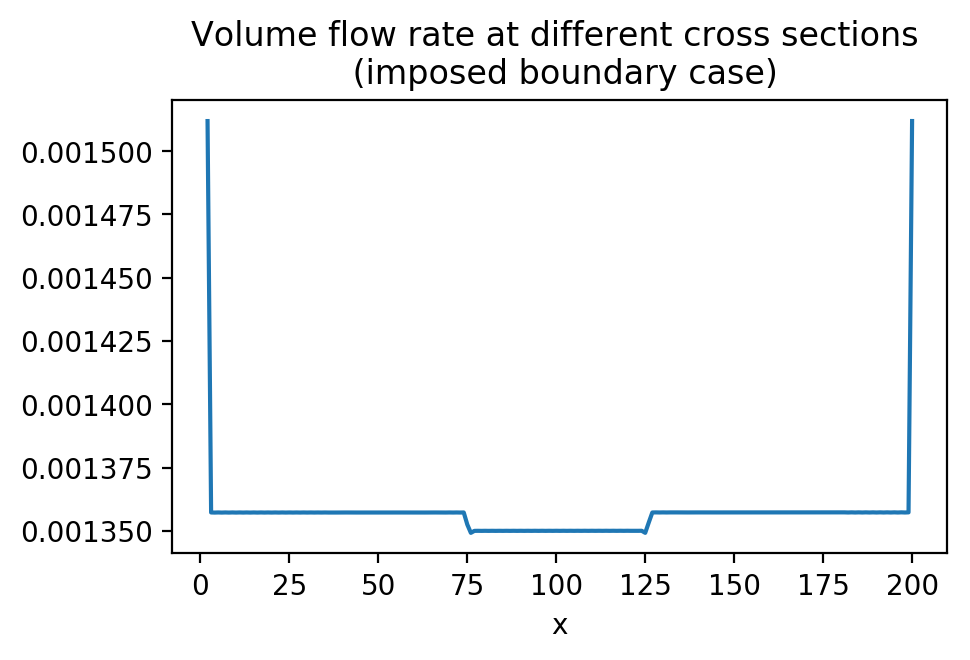
\includegraphics[scale=0.8]{case2_volume_flow}
\centering
\caption{Volume flow rates for non-periodic boundary case}
\label{fig:flow_case2}
\end{figure}

\end{solution}

\begin{solution} 
\textbf{Average Velocity}

The average velocity is $3.45 \times 10^{-5}$ for periodic boundary and $2.61 \times 10^{-5}$ for non-periodic. 

The maximum velocity is $9.30 \times 10^{-5}$ for periodic boundary and $6.98 \times 10^{-5}$ for non-periodic. $u_y$ is orders of magnitude smaller than $u_x$ and has negligible contribution to the total velocity magnitude.

We can further plot the average and maximum velocity at each cross-section $x=x_i$, as shown in Fig \ref{fig:profile_case1} and Fig \ref{fig:profile_case2}. This velocity is significantly higher inside the narrowing region, consistent with the continuity equation of fluid. This result also matches our intuition of the system.

\begin{figure}[H]
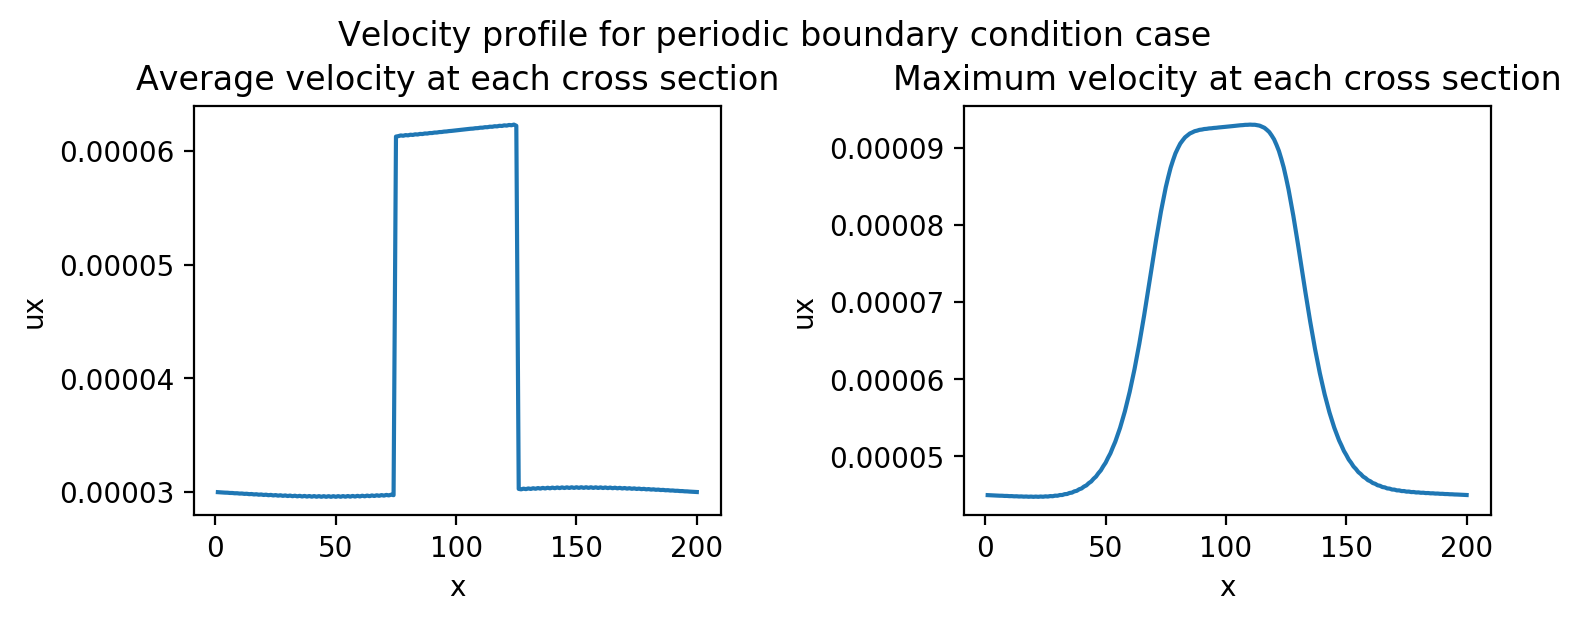
\includegraphics[scale=0.75]{case1_u_profile}
\centering
\caption{Average and maximum velocity at each cross-section, for periodic boundary case}
\label{fig:profile_case1}
\end{figure}

\begin{figure}[H]
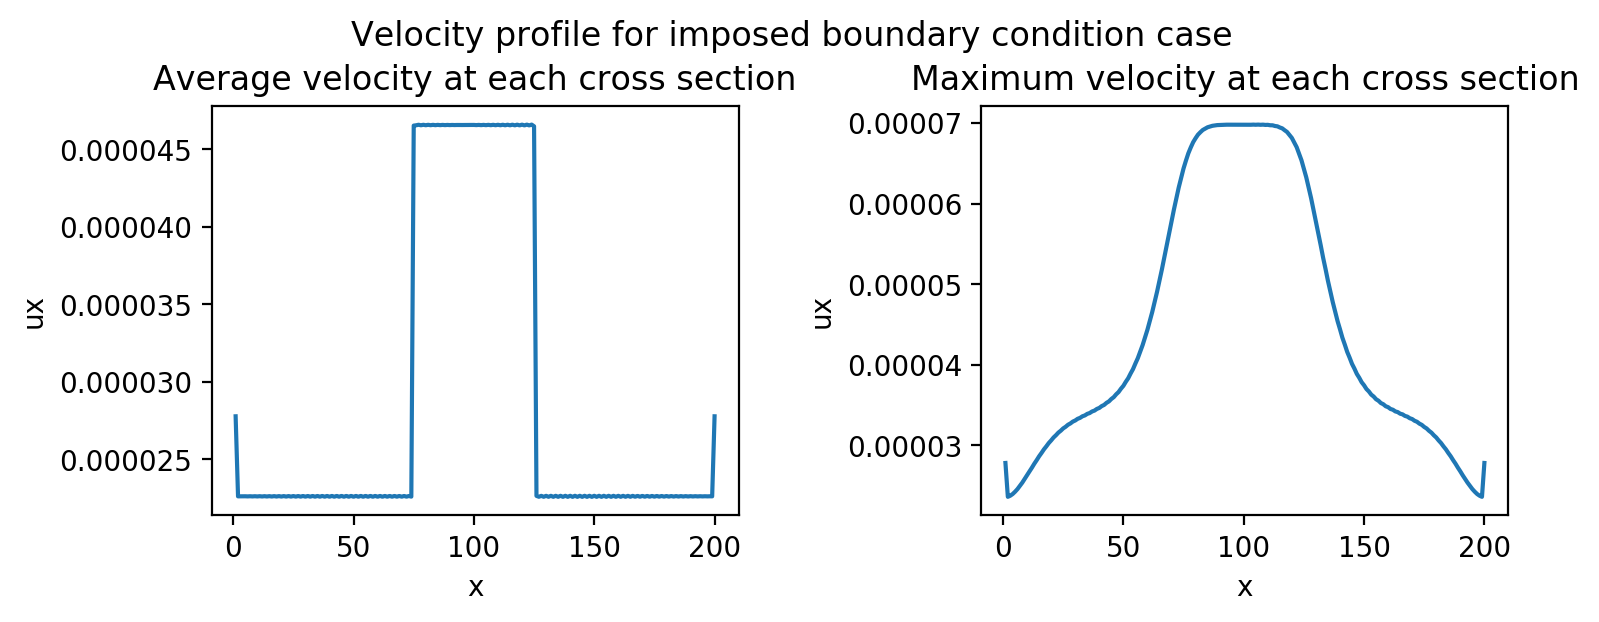
\includegraphics[scale=0.75]{case2_u_profile}
\centering
\caption{Average and maximum velocity at each cross-section, for non-periodic boundary case}
\label{fig:profile_case2}
\end{figure}

\end{solution}

\begin{solution} 

We can further check the velocity profile at each cross-section. For 2D Poiseuille flow without walls, the analytical solution is known to be a parabola. With walls, the shape should still be parabola-like, as confirmed by Fig \ref{fig:profile_case1} and Fig \ref{fig:profile_case2}. Inside the narrowing region ($x=100$), the parabola is the sharpest. The only non-parabola-like profile is the non-periodic boundary case at $x=0$, because we impose uniform velocity at the boundary.

\begin{figure}[H]
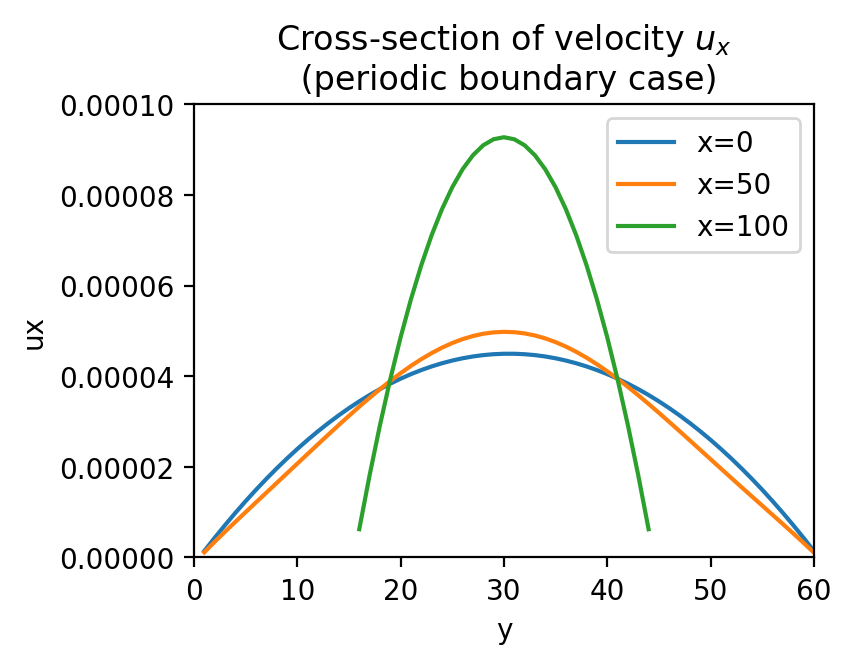
\includegraphics[scale=0.75]{case1_u_cross_section}
\centering
\caption{Velocity profile at three cross-sections, for periodic boundary case.}
\label{fig:profile_case1}
\end{figure}

\begin{figure}[H]
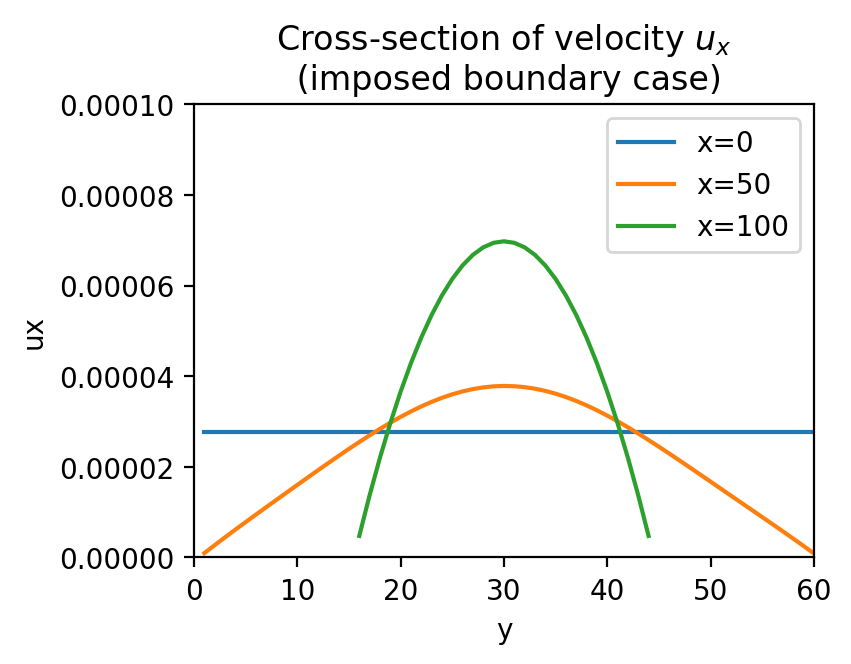
\includegraphics[scale=0.75]{case2_u_cross_section}
\centering
\caption{Velocity profile at three cross-sections, for non-periodic boundary case.}
\label{fig:profile_case2}
\end{figure}

\end{solution}



    Repeat the simulation by varying the width of the narrowing $w$.


    \textbf{Plot:}
    Show how the flow rate changes by varying $w$ in the range $0<w<50$

\graphicspath{ {./JiaweiZhuang/HW2_figures/different_width/} }

\begin{solution} 

Running the simulation with varying sizes of $w=10, 20, 30, 40, 50$, we obtain the following velocity profiles. The steady state velocity $u$ is shown in Fig \ref{fig:ux_ws_case1} and Fig \ref{fig:ux_ws_case2}. The periodic cases has parabola-like velocity profile at the boundary, while the non-periodic we imposed to have uniform profile over $y$ near boundary.

\begin{figure}[H]
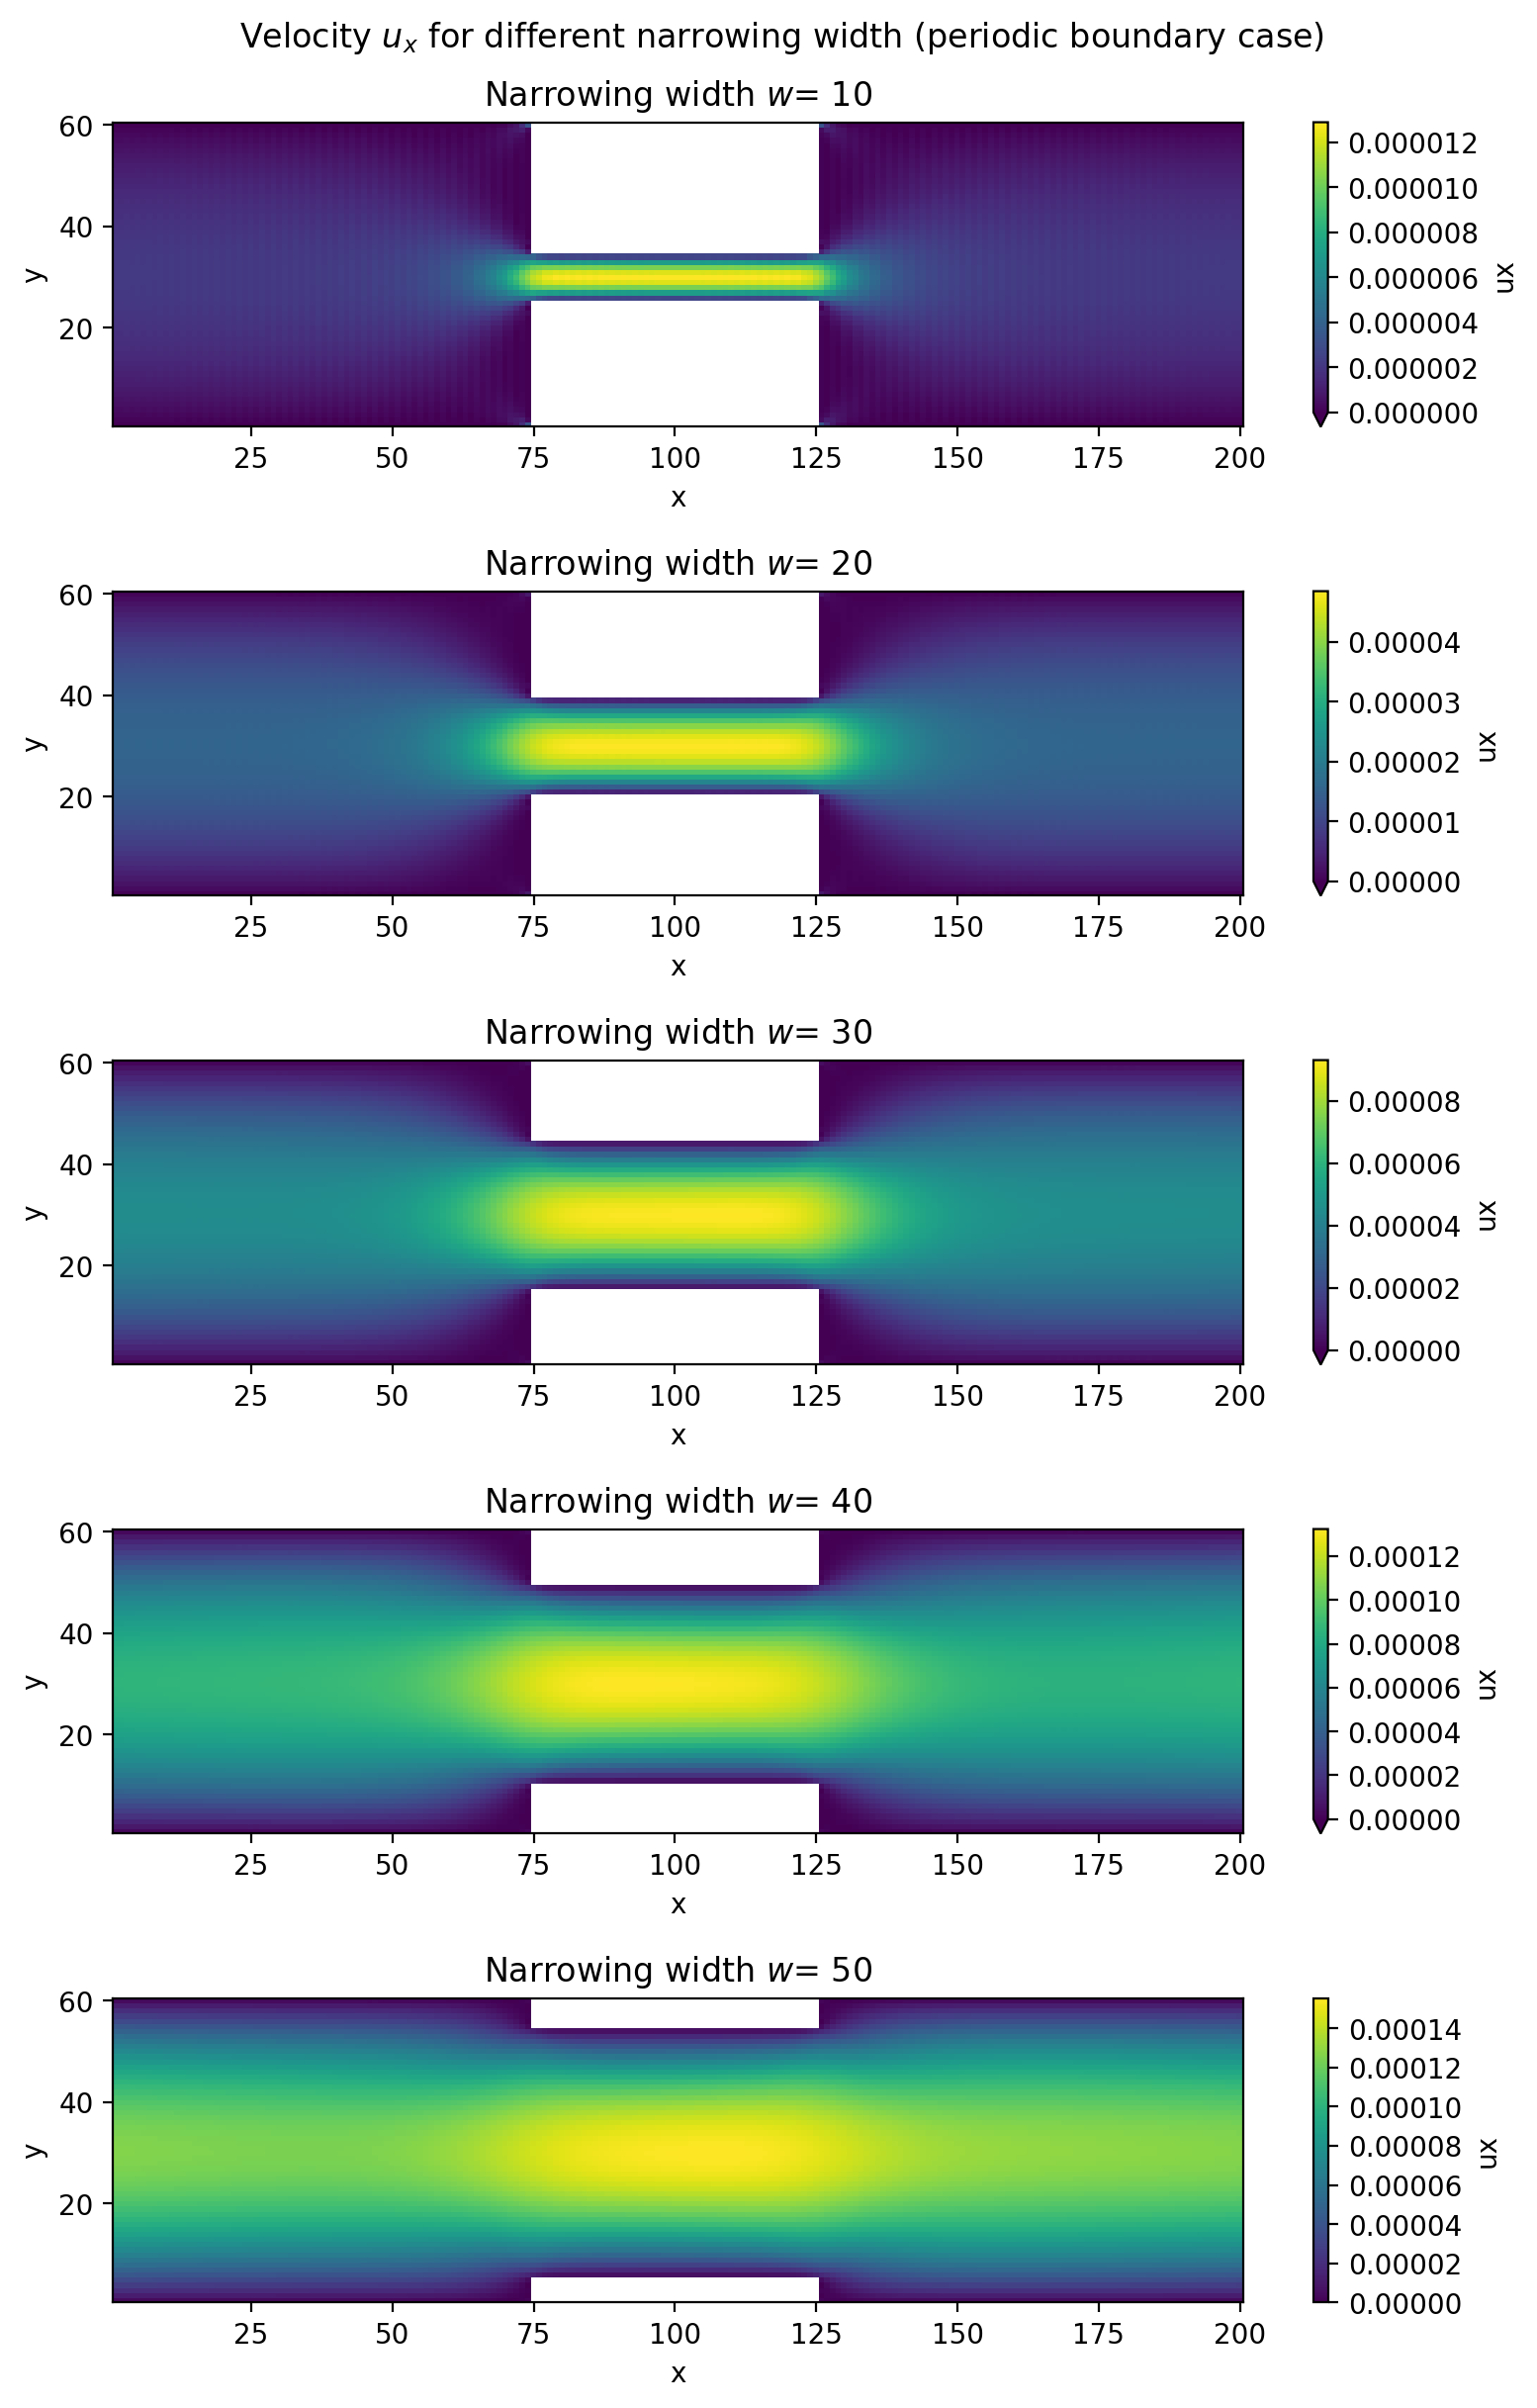
\includegraphics[scale=0.6]{case1_ux_different_width}
\centering
\caption{Velocity field with different narrowing width, for periodic boundary case.}
\label{fig:ux_ws_case1}
\end{figure}

\end{solution}

\begin{solution} 

\begin{figure}[H]
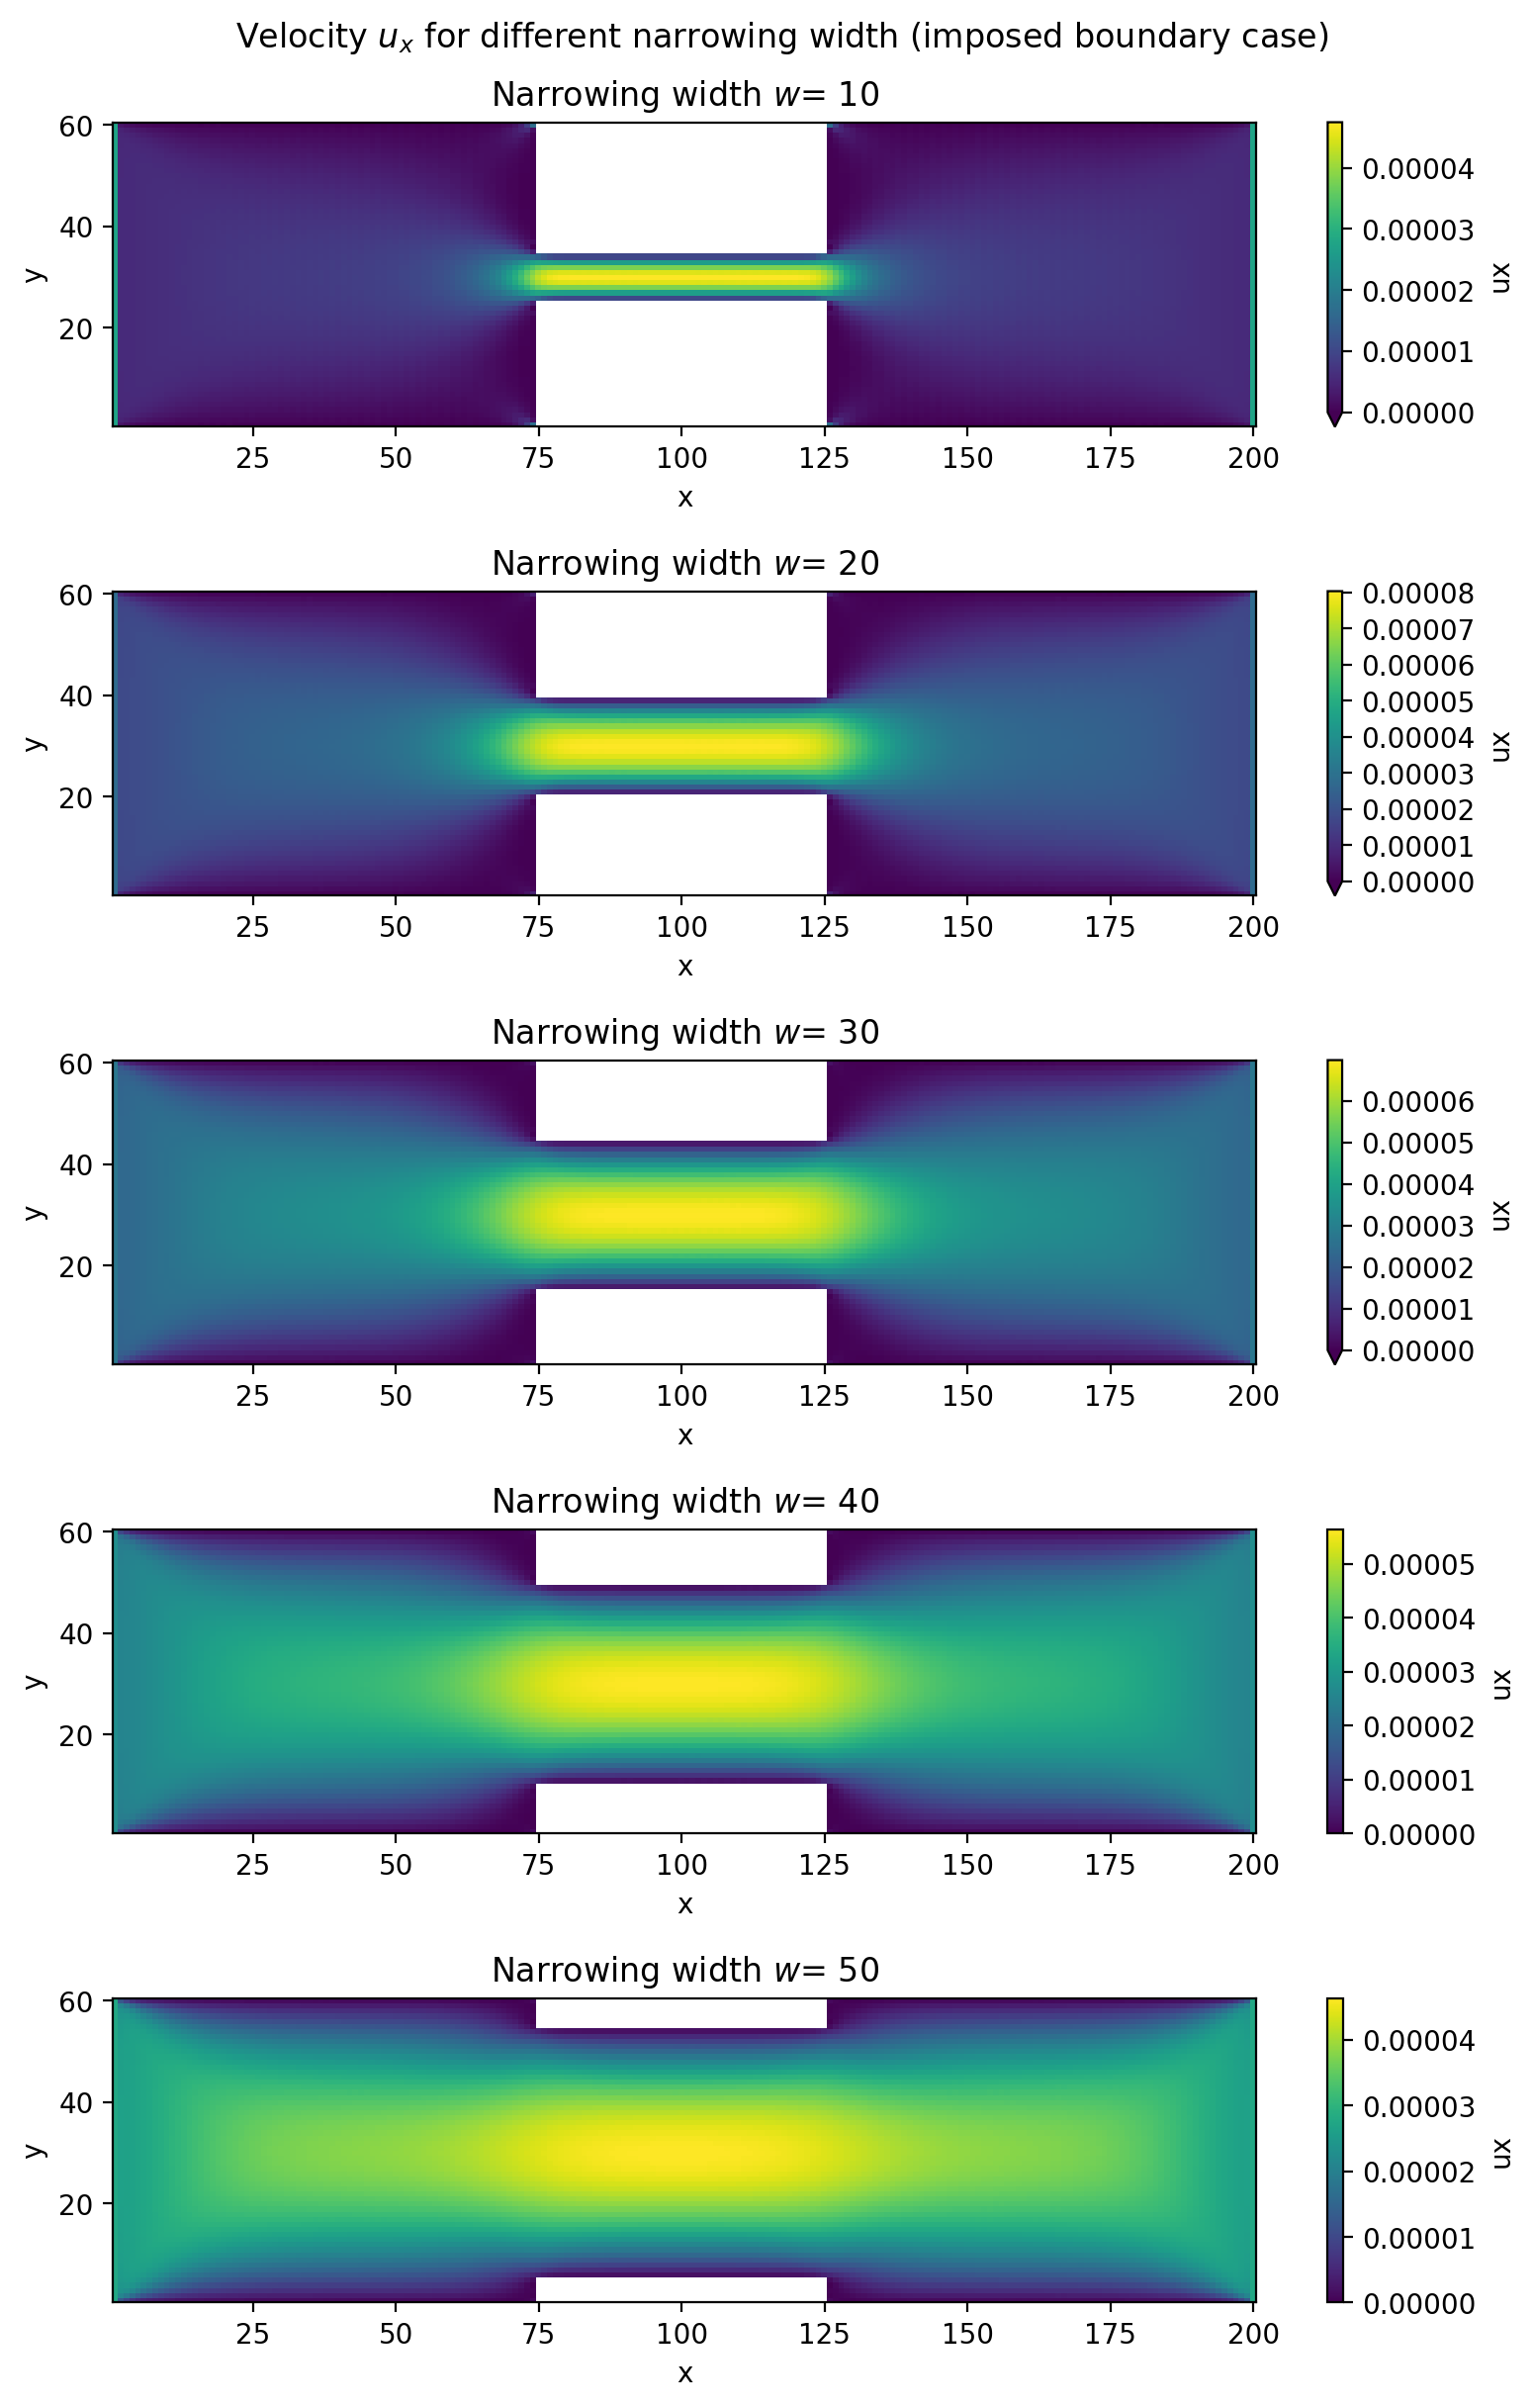
\includegraphics[scale=0.6]{case2_ux_different_width}
\centering
\caption{Velocity field with different narrowing width, for non-periodic boundary case.}
\label{fig:ux_ws_case2}
\end{figure}

\end{solution}


\begin{solution} 

We then compute the volume flow rate by integrating over $y$ and then averaging over $x$. The rates for different $w$ are shown in Fig \ref{fig:flow_ws_case1} and Fig \ref{fig:flow_ws_case2}. In both cases, the rate increases with the channel width, as expected.

\begin{figure}[H]
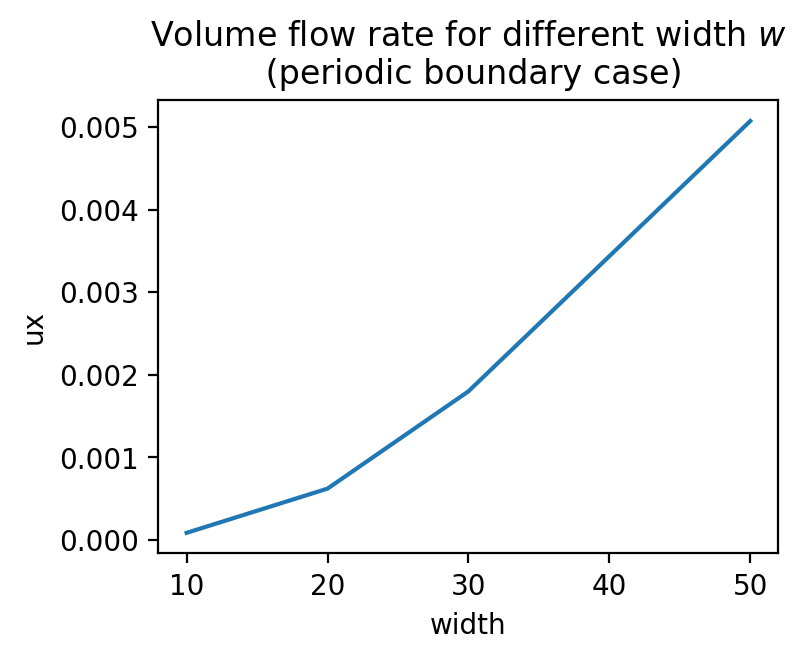
\includegraphics[scale=0.6]{case1_ws_volume_flow}
\centering
\caption{Volume flow rate (averaged) with different narrowing width, for periodic boundary case.}
\label{fig:flow_ws_case1}
\end{figure}

\begin{figure}[H]
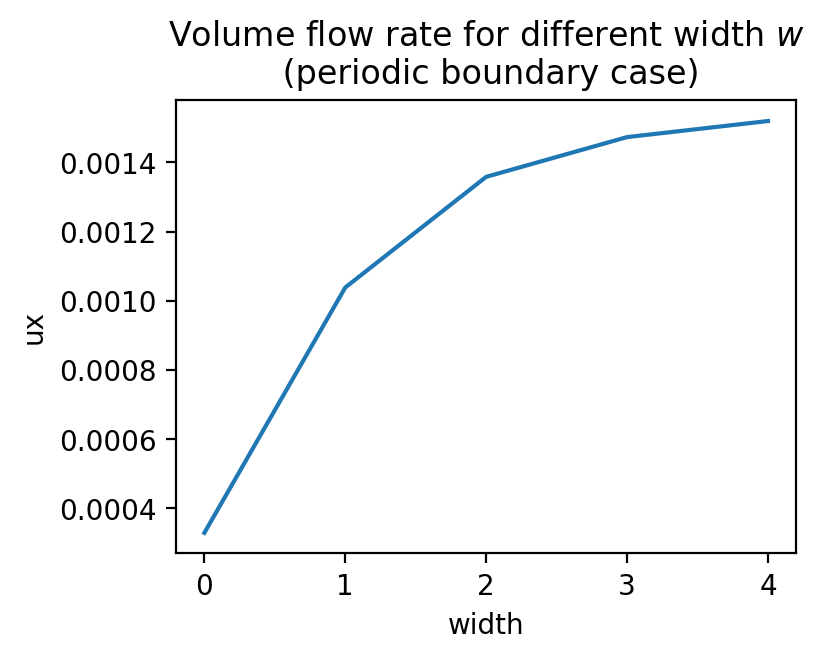
\includegraphics[scale=0.6]{case2_ws_volume_flow}
\centering
\caption{Volume flow rate (averaged) with different narrowing width, for non-periodic boundary case.}
\label{fig:flow_ws_case2}
\end{figure}

\end{solution}

    Compare the pressure at the narrowing with the simple Bernoulli estimate for inviscid flows, stating that
    $$
    \frac{1}{2} \rho u_o^2 + p_o = \frac{1}{2} \rho u_i^2 + p_i
    $$
    where $u_o$ and $p_o$ are cross-sectional averages of velocity and pressure at $x=0$ for a periodic system 
    or at the inlet otherwise, and $u_i$ and $p_i$ are the same quantities at the center of the narrowing. 
    
    \textbf{Plot:}
    Plot the obtained pressure vs the Bernoulli estimate by varying the LBM kinematic viscosity in the range 0.05 : 0.1667.

\graphicspath{ {./JiaweiZhuang/HW2_figures/bernoulli_question/} }

\begin{solution} 

We find that the term $\frac{1}{2} \rho u^2$ is orders of magnitude smaller than the pressure $p$. This is because the velocity $u$ is small (a result of the small Reynolds number). The pressure $p$ is almost constant (only 0.002\% perturbation) over the entire domain. This is demonstrated by Fig \ref{fig:ber_case1} and Fig \ref{fig:ber_case2}, where we can see that $\frac{1}{2} \rho u^2 + p \approx p$. The pressure $p$ is almost $0.166$ everywhere, and the velocity perturbation is negligible. In this case, the Bernoulli estimate almost just uses $p_0$ to approximate $p_i$. The relative error is less than 0.002\%.

\begin{figure}[H]
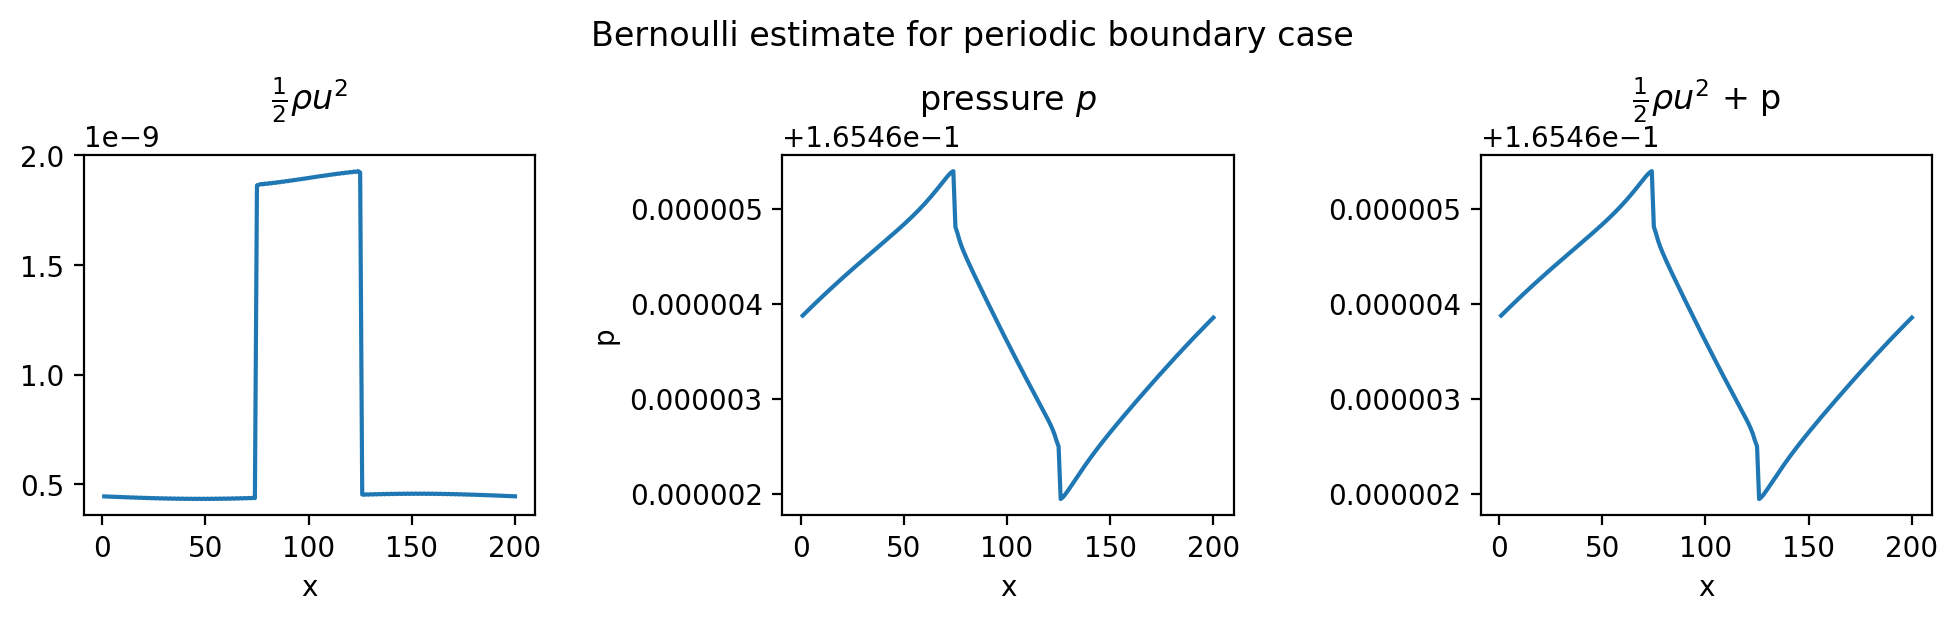
\includegraphics[scale=0.6]{bernoulli_case1_default}
\centering
\caption{Major quantities used in Bernoulli estimate, for periodic boundary case.}
\label{fig:ber_case1}
\end{figure}

\begin{figure}[H]
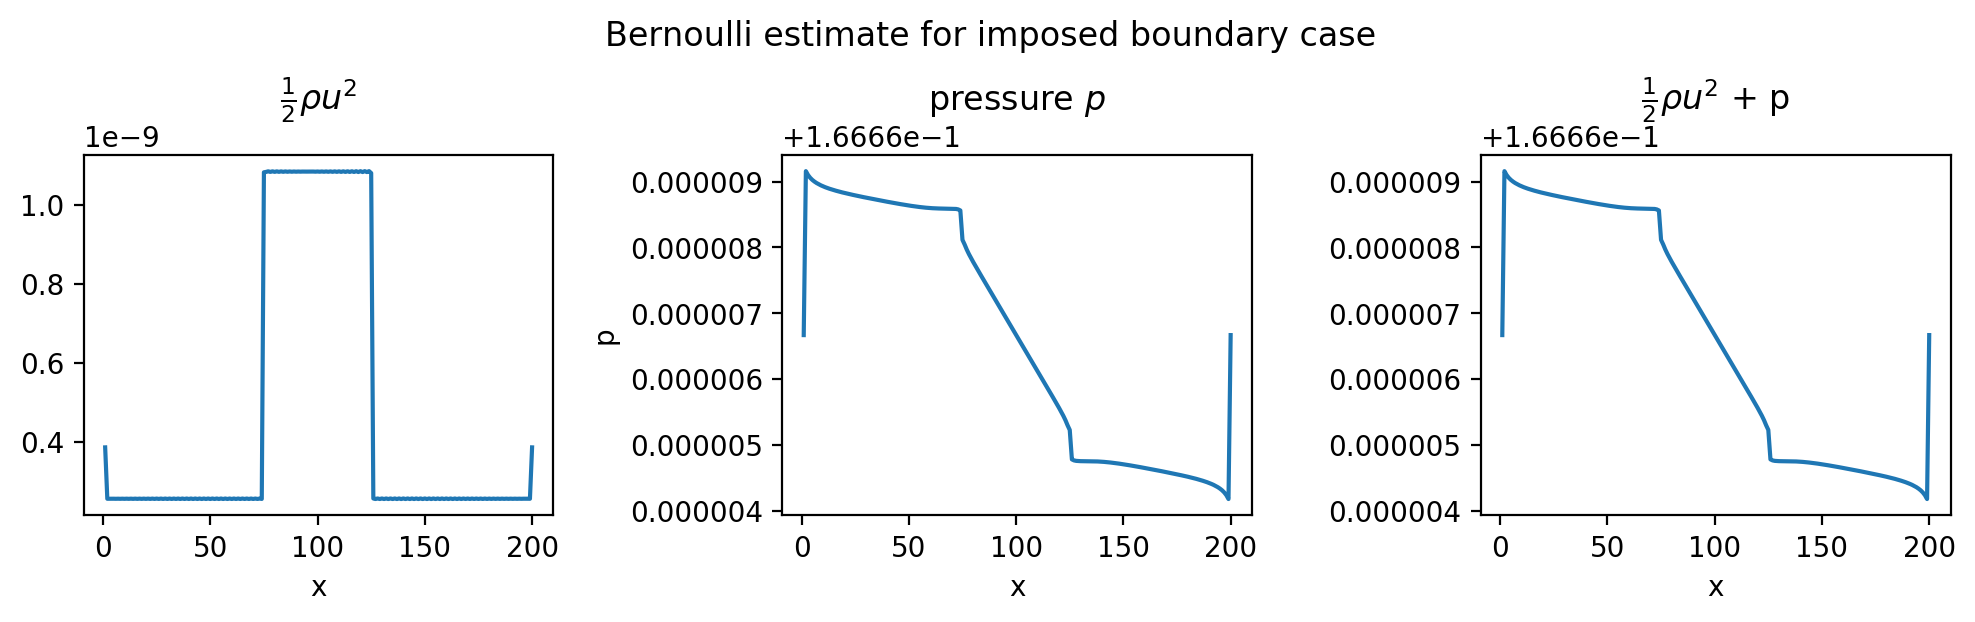
\includegraphics[scale=0.6]{bernoulli_case2_default}
\centering
\caption{Major quantities used in Bernoulli estimate, for non-periodic boundary case.}
\label{fig:ber_case2}
\end{figure}

\end{solution}


\begin{solution} 

Finally, we vary the LBM kinematic viscosity by tweaking the relaxation parameters $\Omega$. For all the previous cases we set $\Omega=1.0$, thus $\nu=1/6=0.1667$, which is the upper bound of $\nu$. For the lower bound $\nu=0.05$, the corresponding $\Omega = 1.54$. The velocity fields with different viscosity are shown in Fig \ref{fig:u_case1_nus}. Smaller viscosity leads to higher velocity magnitude, as expected.

\begin{figure}[H]
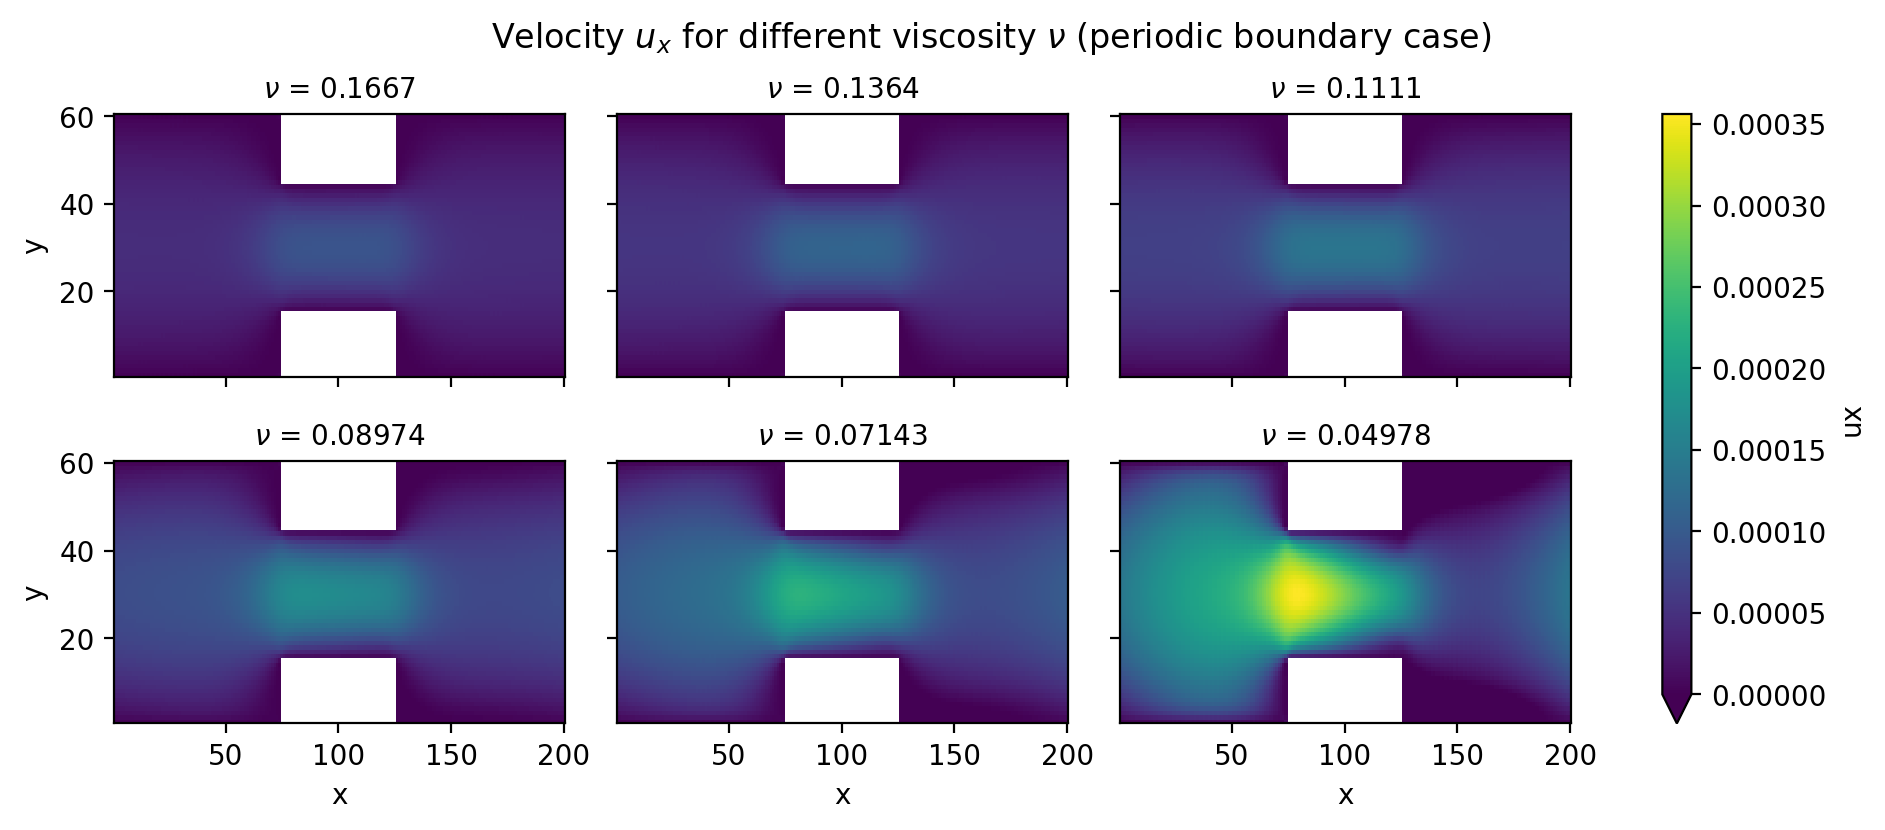
\includegraphics[scale=0.62]{u_case1_nus}
\centering
\caption{Velocity field for different viscosity $\nu$. Here uses Periodic boundary. The non-periodic one has similar behavior.}
\label{fig:u_case1_nus}
\end{figure}

For different viscosity $\nu$, the Bernoulli estimate has similar behavior, as shown in Fig \ref{fig:u_case1_nus}. The kinetic energy term $\frac{1}{2} \rho u^2$ becomes smaller with higher viscosity, as expected. The pressure term $p$, however, stays almost constant, and dominates the total term $\frac{1}{2} \rho u^2 + p$.

\begin{figure}[H]
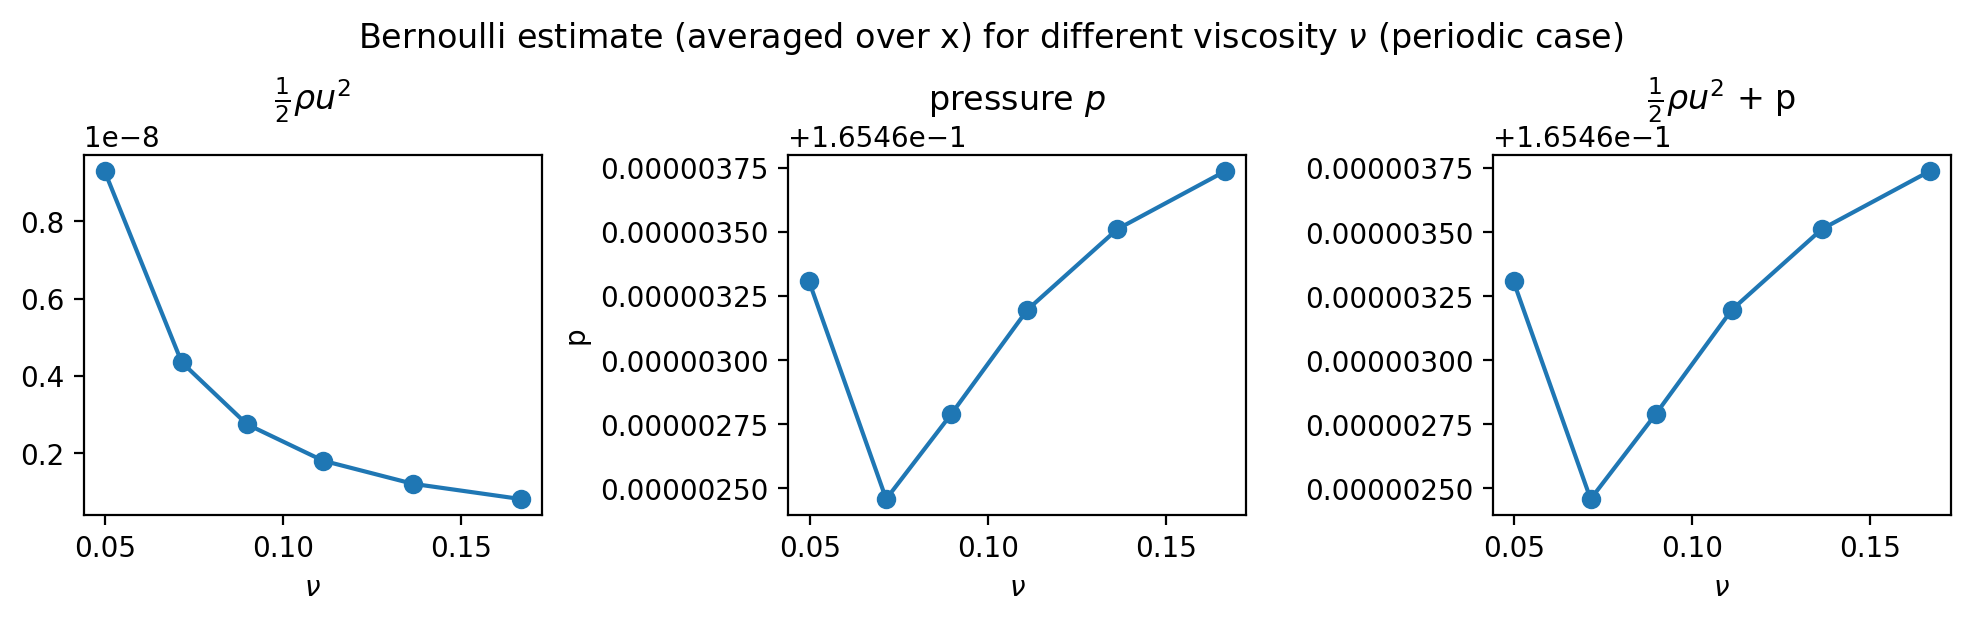
\includegraphics[scale=0.62]{bernoulli_case1_nus}
\centering
\caption{Major quantities used in Bernoulli estimate (averaged over x), for different viscosity $\nu$. Here uses Periodic boundary. The non-periodic one has similar behavior.}
\label{fig:bernoulli_case1_nus}
\end{figure}

\end{solution}


\begin{solution} 

All figures can generated by the Python notebook JiaweiZhuang/use\_LBM\_solver.ipynb.

\end{solution}

\begin{solution}
In conclusion, we simulated a periodic channel and a non-periodic channel using the LBM. The results were computed rather quickly   highlighting the efficiency of the LBM at producing reliable results when simulating flows.\\
\\
To test the validity of our approach and design for implementing LBM we originally coded our design in Python. The results appeared accurate and held to the boundary conditions we constrained the problem to. Additionally, the organization that we used for the code follows that of Sauro Succi. We then translated our code and methods to C in order to achieve more efficient computational speeds enabling us to run our LBM to higher iteration numbers quicker for both cases. We interpreted the output of the C method in Python for better visualization using various libraries. \\
\\
The periodic channel can be found on the file "LBM\_2D\_channel\_v1.c" and the continuous channel can be found in the file "LBM\_2D\_channel\_v2.c". In the files one can change various parameters associated with the environment that the flow is in such as H, L, w, l, the forces, etc. 
\end{solution}

%%% PROBLEM 2 %%%
  \section{Problem 2:  Basic CUDA and GPUs}
    \textit{This problem was submitted by Dan Willen \texttt{daniel.p.willen@gmail.com}}

    Consider the equation
    \begin{equation}\label{eq:heat}
      \frac{\partial u}{\partial t} = D \nabla^2 u,
    \end{equation}
    on the domain \(0 \leq x,y \leq \pi\), with \(u = u(x,y,t)\), \(D\) the diffusive constant, and \(\nabla^2\) the Laplace operator.
    The boundary conditions are of the homogeneous Dirichlet type:
    \begin{equation}
      u(x = 0, y) = u(x = \pi, y) = u(x, y = 0) = u(x, y = \pi) = 0,
    \end{equation}
    and the initial condition is
    \begin{equation}
      u(x,y, t = 0) = \sin(x) \sin(y).
    \end{equation}
    The solution to this equation is
    \begin{equation}
      u(x,y,t) = \sin(x) \sin(y) \exp{(-2Dt)}
    \end{equation}
    
    Using a second-order central difference in space and first order forward difference in time, the discretization of \eqref{eq:heat} is
    \begin{equation}
      u_{i,j}^{\left(n+1\right)} = u_{i,j}^{\left(n\right)} + \frac{D \Delta t}{\Delta x^2} 
        \left[u_{i+1, j}^{\left(n\right)} +
              u_{i-1, j}^{\left(n\right)} +
              u_{i, j+1}^{\left(n\right)} +
              u_{i, j-1}^{\left(n\right)} -
              4u_{i, j}^{\left(n\right)} \right],
    \end{equation}
    where \(u_{i,j}^{\left(n\right)}\) is the value of \(u\) at the \(n^{th}\) time step at grid point \((i,j)\), \(\Delta t = \Delta x^2 / 4D\) is the time step size, and \(\Delta x\) is the grid spacing in the \(x\) and \(y\) directions.
    
    \vspace{5mm}
    
    \begin{enumerate}
      \item Using Cuda, solve the discretized equations up to a time \(t = \pi^2/D\) using the Jacobi method.
        A skeleton code is provided to assist you, with comments in the locations you should make changes.
        \begin{enumerate}[Step I --]
          \item Declare, allocate, and initialize memory for the field variable \texttt{u} on the CPU.
            You should allocate enough memory for the grid, which has size \(nx \times ny\) and initialize \texttt{u} to the initial condition.
            Make sure you free the memory at the end of the program.
          \item Declare and allocate the GPU memory for \texttt{\_u}, \texttt{\_u\_new}\, and \texttt{\_error}.
            Copy the CPU memory to the GPU; the other two arrays have been initialized to zero for you.
            Make sure you free the memory at the end of the program.
          \item Set up the kernel execution configuration for the GPU kernel based on the input domain size and the maximum threads per dimension,
            which is set at the top of the file as a \texttt{\#define}.
            You will need to determine the number of threads per block and the number of blocks in each direction, as well as set up the \texttt{dim3} variables.
          \item Write a GPU kernel that advances to the next timestep using the Jacobi method.
            This should be done in parallel, not in serial.
          \item Write a GPU kernel that calculates the error between the numerical and analytic solutions at each point.
            Be careful to compare solutions at the correct timestep -- \texttt{\_u\_new} is at \(t = (n+1) \Delta t\) and \texttt{\_u} is at \(t = n \Delta t\).
            Using this result, a parallel reduction using the Thrust parallel algorithms library has been provided to calculate the total error in order to find the average percent error at each grid point.
          \item At the end of the loop, copy the data back to the CPU.
        \end{enumerate}
    \end{enumerate}
    
    Your program should take as an input the number of grid cells on one side of the domain.
    This has been set up for you such that the program can be run from the command line like: 
    \vspace{3mm}\\ \texttt{./jacobi\_solver.cu n} \vspace{3mm}\\
    where \(nx = ny = \) \texttt{n} is the size of one side of the square domain.
    The program should output the percent difference between your result and the analytic solution, averaged over all of the grid nodes:
    \begin{equation}
      \epsilon = \frac{1}{n_x n_y} \sum_{i=1}^{n_x} \sum_{j=1}^{n_y} \frac{u_{i,j}^{\left(n\right)} -
U_{i,j}^{\left(n\right)}}{U_{i,j}^{\left(n\right)}},
    \end{equation}
    where \(U\) is the analytic solution.
    
    If you have time, discuss the following:
    \begin{itemize}
      \item How does the error change as you increase the resolution? Does this behavior make sense?
      \item How does the runtime scale with the resolution? You can get a rough estimate by using the bash command \texttt{time} when executing your program, like:
    \vspace{3mm}\\ \texttt{./jacobi\_solver.cu n} \vspace{3mm}\\ and using the result for \texttt{real}. \\
      \item How does the runtime change as you change the kernel execution configuration?
        e.g., play around the \texttt{MAX\_THREADS\_DIM} parameter as well as different schemes for setting up the thread blocks.
      \item Use shared memory in the Jacobi kernel
    \end{itemize}

\begin{solution}

We developed the code based on the skeleton provided in \texttt{parallel.cu}. 
In addition to the basic requirements stated in the 5 steps in the problem statement, we used the constant memory and the shared memory to accelerate the computation. 
In particular, the constant memory is applied to store the constant variables such as \texttt{nx} and \texttt{ny}, and the shared memory is applied to cache the field variable \texttt{\_u} as each of its element would be accessed for multiple times by different threads in one Jacobi iteration. 
Our completed code has been uploaded  \href{https://github.com/iacs-ac290r-2019-2/homework/tree/master/HW2/Group/Problem2}{here}. 
\\
The code is compiled and tested on Odyssey, the HPC cluster maintained by Harvard FAS Research Computing. We observed how the performance scale with the resolution as well as the block dimension. The results are displayed in Figure \ref{fig:p2_res} and Figure \ref{fig:p2_thr}. 

\begin{figure}[H]
    \centering
    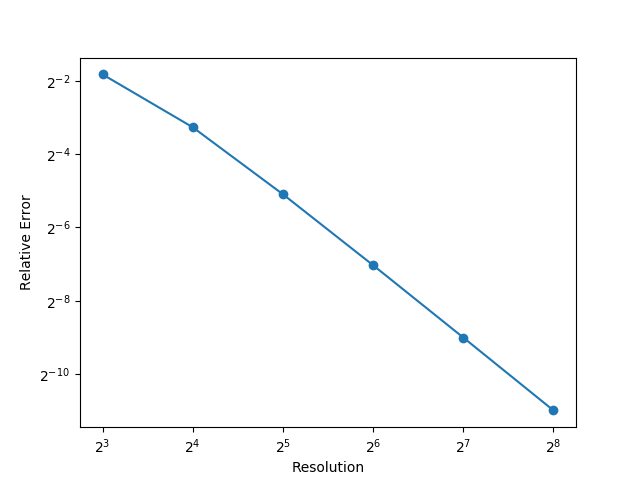
\includegraphics[scale=0.4]{YiqiXie/res_err.png}
    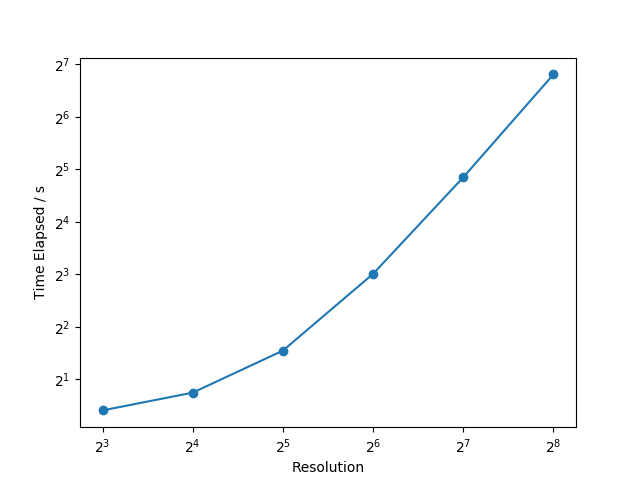
\includegraphics[scale=0.4]{YiqiXie/res_time.png}
    \caption{Performance scale with the resolution. \texttt{MAX\_THREAD\_NUM}=18. }
    \label{fig:p2_res}
\end{figure}

\begin{figure}[H]
    \centering
    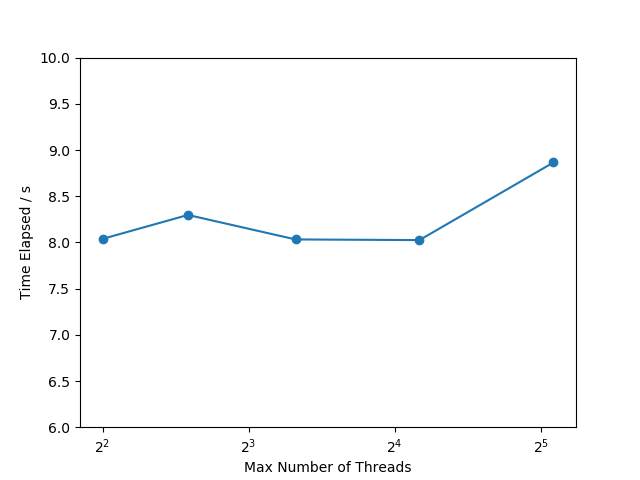
\includegraphics[scale=0.4]{YiqiXie/thr_time.png}
    \caption{Performance scale with the block dimension. The grid is $64\times 64$. }
    \label{fig:p2_thr}
\end{figure}

As we enhance the resolution (denoted by the grid size $N\times N$), we see that the relative error shrinks asymptotically with $O(\frac{1}{N^2})$, and the elapsed time increases asymptotically with $O(N^2)$, which makes sense for our Jacobi iteration setup. On the other hand, the performance does not seem to vary a lot with block dimension. Due to hardware restriction, we cannot try $\texttt{MAX\_THREADS\_DIM}\geq 2^6$. Based on the trend in Figure \ref{fig:p2_thr}, the runtime might increase with larger block dimensions. 

\end{solution}

\end{document}

